\documentclass[11pt]{article}
\usepackage[T1]{fontenc}
\usepackage{lmodern,microtype}
\usepackage[a4paper,margin=28mm]{geometry}
\usepackage{amsmath,amssymb,amsthm,mathtools,booktabs,array,xurl}
\usepackage{tikz}
\usetikzlibrary{arrows.meta,calc,patterns}
\usepackage[colorlinks=true,linkcolor=blue!55!black,citecolor=blue!55!black,urlcolor=blue!55!black]{hyperref}
\numberwithin{equation}{section}
\setlength{\emergencystretch}{2em}
\newtheorem{theorem}{Theorem}[section]
\newtheorem{proposition}[theorem]{Proposition}
\newtheorem{lemma}[theorem]{Lemma}
\newtheorem{corollary}[theorem]{Corollary}
\theoremstyle{definition}
\newtheorem{definition}[theorem]{Definition}
\theoremstyle{remark}
\newtheorem{remark}[theorem]{Remark}
\newcommand{\ii}{\mathrm i}
\newcommand{\Rea}{\operatorname{Re}}
\newcommand{\Ima}{\operatorname{Im}}
\newcommand{\Vol}{\operatorname{Vol}}
\newcommand{\arsinh}{\operatorname{arsinh}}
\newcommand{\artanh}{\operatorname{artanh}}
\newcommand{\PSL}{\operatorname{PSL}}
\newcommand{\calC}{\mathcal C}
\title{Positive octahedra and primitive fillings\protect\\for trees of crossing circles}
\author{}
\date{}
\begin{document}
\maketitle

\begin{abstract}
An ordered tree of crossing circles has two ideal octahedra for each
physical quarter-turn in its tangle construction. We give explicit
holomorphic shapes for these cells and follow the original peripheral
curves through their gluing. If a circle has degree $d_v$ and is filled
to crossing power $n_v$, the condition
$\sqrt{d_v^2+n_v^2}\ge630$ at every circle produces a positive cone
deformation from the augmented exterior to the smooth filled exterior.
The bound is independent of the number of circles and allows zero
powers at sufficiently large degrees. We identify the absolute metric
volume with a holomorphic critical action, bound the core lengths and
volume loss, and give a more flexible criterion with a different
parameter radius at each vertex. The argument concerns the original
marked link complement and does not require a quantum asymptotic.
\end{abstract}

\section{The marked diagrams and the geometric statement}
\label{ctg:introduction}

A crossing circle is an auxiliary component surrounding two strands;
its spanning disk is punctured twice by those strands. Removing full
twists while retaining the circle gives an augmented link. Filling the
circle along its disk-framed slope restores the original twists.
The marking of that slope matters: a full turn and a trivial endpoint
permutation are different operations.

We use two-string tangles with four ordered endpoints, vertical
stacking, a physical quarter-turn $T$, and cylindrical closure $C$.
The underlying finite tree $\mathcal T$ has at least one edge. Each
vertex carries its own crossing-circle tangle $P_v$; there are no bare
product junctions. In a rooted description, a nonroot tangle is
\begin{equation}\label{ctg:word}
 W_v=\left(\prod_{w\in I_v^-}T(W_w)\right)P_v
             \left(\prod_{w\in I_v^+}T(W_w)\right).
\end{equation}
The two lists have their specified order and record the cut at the
parent edge in the original cyclic order. One may choose a terminal
root and close its tangle with the adjacent turned branch. All rotations
of child balls, endpoint frames, and disk orientations are retained.
In particular a double turn is the physical half-turn, which reverses
the order of a stack; it is not erased by a scalar identity.

Let $e$ be the number of tree edges, and $d_v\ge1$ the degree of vertex
$v$. Choose $\epsilon_v\in\{-1,0,1\}$ and an integer $p_v$, and put
\begin{equation}\label{ctg:powers}
 n_v=\epsilon_v-2p_v.
\end{equation}
The augmented diagram retains the crossing $R^{\epsilon_v}$ in the
original local frame. Its exterior is denoted $Y^\epsilon$. The original
meridian $\mu_v$ and disk longitude $\lambda_v$ form a primitive basis
on the crossing-circle torus. Our sign convention for $R$ is that
filling $\mu_v+p_v\lambda_v$ restores $R^{n_v}$. Section~\ref{ctg:words}
specifies the two odd meridian words, so this convention includes both
signs of a retained half twist. To see the underlying surgery, cut
along the twice-punctured disk and rotate one side through $p_v$ full
turns before removing the auxiliary circle. The slope becomes the
meridian of the added solid torus, and the two strands acquire
$-2p_v$ crossings in this disk frame. This local operation takes
place in a ball in $S^3$; it does not change the ambient manifold.
Write $Y(\mathbf p)$ for the result of
filling only these auxiliary tori. The main components are the strands
left after filling. Their number is determined by the literal endpoint
matching, not by the abstract tree. If that matching gives one component,
write it as $K_{\mathbf n}$; then $Y(\mathbf p)=S^3\setminus K_{\mathbf n}$.

Let $v_{\rm oct}$ be the volume of a regular ideal octahedron. For
complex $t,u$ near zero define the holomorphic function $\psi$ by
\begin{equation}\label{ctg:psi}
 \psi(0,0)=\frac{v_{\rm oct}}{\pi},\qquad
 \psi_t(t,u)=-\frac1\pi\arsinh\!\left(\tan(t/2)\cos(u/2)\right),
 \qquad \psi_u(t,u)=\psi_t(u,t).
\end{equation}
All branches continue from zero. The equality of the cross derivatives,
proved in Section~\ref{ctg:contraction}, makes this a definition rather
than an extra existence assumption. Put
\[
 \Psi(\boldsymbol\tau)=\sum_{vw\in E(\mathcal T)}\psi(\tau_v,\tau_w),
 \qquad L_v=\sqrt{d_v^2+n_v^2},\qquad \delta=\frac1{39000}.
\]

\begin{theorem}\label{ctg:main}
For the marked diagrams above, suppose $L_v\ge630$ for every vertex.
There is a unique solution in $|\tau_v|\le10^{-2}$ of
\begin{equation}\label{ctg:charge}
 \Psi_{\tau_v}(\boldsymbol\tau)+\frac{\ii n_v}{2\pi}\tau_v=\ii c.
\end{equation}
It is holomorphic in $c$ on a neighborhood of the closed unit disk,
vanishes at $c=0$, and for real $0<c\le1$ satisfies
\begin{equation}\label{ctg:tau-bound}
 |\tau_v(c)|\le\frac{2\pi c}{L_v-\delta d_v},
 \qquad \Ima\tau_v(c)<0.
\end{equation}
The original augmented exterior admits a positive ideal-cell metric
with auxiliary logarithmic periods
\begin{equation}\label{ctg:periods}
 U_v=-2\pi\Psi_{\tau_v}-\ii\epsilon_v\tau_v,
 \qquad V_v=2\ii\tau_v,
 \qquad U_v+p_vV_v=-2\pi\ii c.
\end{equation}
These are the full periods of the primitive curves, continued from
completeness. Completing the auxiliary ends gives cone angle $2\pi c$
and core length $\ell_v(c)=-2\Ima\tau_v(c)$. At $c=1$ the completion is
smooth, complete, and of finite volume on $Y(\mathbf p)$; all main
cusps remain complete.

Define the stationary value, at the solution of \eqref{ctg:charge},
\begin{equation}\label{ctg:action}
 \calC(c)=\Psi(\boldsymbol\tau(c))
       +\frac{\ii}{4\pi}\sum_vn_v\tau_v(c)^2
       -\ii c\sum_v\tau_v(c).
\end{equation}
The absolute volume of the completed cone metric is
\begin{equation}\label{ctg:volume}
 \Vol_c=2\pi\Rea\calC(c),\qquad
 \Vol_0=2e\,v_{\rm oct}.
\end{equation}
In particular, if the main component is a knot, the right side at
$c=1$ is $\Vol(S^3\setminus K_{\mathbf n})$.
\end{theorem}

The theorem is a sufficient geometric criterion for each fixed finite
diagram. There is no bound on its size, no restriction on the signs of
$n_v$, and no lower bound on $|n_v|$ alone. A vertex with $n_v=0$ is
allowed when $d_v\ge630$. The conclusion does not assert a quantum
invariant limit: that requires an additional finite-source identity
and a noncancellation estimate. Nor is this a theorem about every
strict Conway presentation; the presence of a crossing circle at each
product junction is part of the construction.

The geometry of augmented links, their crossing-disk decompositions,
and the role of regular octahedra are described by Purcell
\cite{Purcell}. Gluing along thrice-punctured spheres has a substantial
history; see Morgan--Ransom--Spyropoulos--Trapp--Ziegler
\cite{BeltedSums} for a recent account of belted decompositions.
We prove the ordered cut and its peripheral markings directly here.
The only specialized companion input is the local peripheral-volume
differential of \cite[Section~7, equation~(7.3)]{MarkedFillings};
its hypotheses and conventions are stated in
Section~\ref{ctg:regulator}. In particular we do not invoke that
paper's independently long-filling theorem.

\section{The projection cut and its ordered octahedra}
\label{ctg:topology}

Opening the projection regions and crossing disks gives two projection
copies. We call disk-side faces shaded and projection faces white.
An ideal vertex records either a main strand segment or an auxiliary
semicircle. The following explicit construction identifies the cut
with the original diagram before any shape is assigned.

For a turned leaf $h_v=T(P_v)$ label its half-segments
\[
 (v_0,v_1,v_2,v_3)
  =(\text{lower left},\text{lower right},\text{upper right},\text{upper left}).
\]
A lower factor $F$ followed by an upper factor $G$ joins $F_2$ to
$G_1$ and $F_3$ to $G_0$, leaving the tuple $(F_0,F_1,G_2,G_3)$.
Closure joins positions $0$ to $3$ and $1$ to $2$. These are empty
joining strips in the projection plane. The inverse turn
$P_v=T^{-1}(h_v)$ has exposed tuple $(v_3,v_0,v_1,v_2)$.

Let $O_v$ denote the auxiliary ideal vertex. Its two shaded triangles
are
\begin{equation}\label{ctg:leaf-faces}
 (O_v,v_1,v_2),\qquad (O_v,v_3,v_0).
\end{equation}
A half-segment in this notation means the ideal vertex containing its
matched pair. The cyclic order around $O_v$ is $(v_0,v_1,v_2,v_3)$.
At a main vertex the corner sectors concatenate in the order of the
planar joining strip. Following the complementary sectors gives all
white face cycles. This determines the oriented boundary ribbon graph,
including more information than just the numbers of faces or components.

The cut is reversible. An auxiliary semicircle is boundary-parallel
in its projection half-ball. Drilling it creates a handle, and opening
its recorded half disk cancels that handle. The disjoint leaf boxes
allow these operations simultaneously. Regluing the white faces by
their projection labels and the shaded faces by their original disk
maps restores the original exterior. A retained half twist changes
the disk regluing, not this open cut.

\begin{proposition}\label{ctg:cut}
Each projection copy is a ball obtained by attaching $e$ octahedra
along $e-1$ triangular faces. Every edge of $\mathcal T$ contributes
one octahedron in each copy. At vertex $v$ the incident blocks give
$d_v$ consecutive disk-side pages, of which exactly one cyclic seam
carries the original retained crossing $R^{\epsilon_v}$.
All main segments, disk curves, and white face cycles agree with
the original marked exterior.
\end{proposition}

\begin{proof}
Consider insertion of a terminal child $h_w$ immediately after $P_v$.
If $x_1,x_2$ are the outside partners of $v_1,v_2$, the product rule is
\begin{equation}\label{ctg:right-insertion}
\begin{array}{c|c}
 \text{before}&\text{after}\\\hline
 v_1-x_1&v_1-w_1,\quad w_2-x_1\\
 v_2-x_2&v_2-w_0,\quad w_3-x_2.
\end{array}
\end{equation}
Write $C=(v_1,x_1)$ and $B=(v_2,x_2)$ for the old vertices. After
insertion these are $(w_2,x_1)$ and $(w_3,x_2)$; the new vertices are
$D=(v_1,w_1)$ and $A=(v_2,w_0)$. Attach an octahedron with apices
$O_v,O_w$, equator $(A,B,C,D)$, and shaded faces
\begin{equation}\label{ctg:oct-faces}
 (O_v,B,C),\quad (O_v,D,A),\quad (O_w,D,C),\quad (O_w,B,A).
\end{equation}
Its first face is glued to the old face $(O_v,C,B)$ with opposite
orientation. The remaining three faces are exactly the new faces
specified by \eqref{ctg:leaf-faces}. The other shaded face at $v$
is unchanged.

The four complementary faces are white triangles. At $B,C,O_v$ remove
the glued shaded sectors and concatenate the remaining sectors.
Their cyclic orders are precisely those of the two strip replacements
in \eqref{ctg:right-insertion}; the new vertices $A,D$ are the two
new identity strips. Consequently the white boundary walks also agree.
Doing the same in the other projection copy adds one pair of
octahedra and one original circle. It introduces no auxiliary circle
at the triangular interface.

Insertion before $P_v$ uses the other face and the equally explicit
table
\begin{equation}\label{ctg:left-insertion}
 v_3-x_3\longmapsto(v_3-w_3,w_0-x_3),\qquad
 v_0-x_0\longmapsto(v_0-w_2,w_1-x_0).
\end{equation}
This follows from the same product rule in the inverse-turn tuple.
Both constructions are reversible by deleting the terminal octahedron.

For the initial edge the two-leaf endpoint matching gives exactly
\eqref{ctg:oct-faces} in each projection copy. Choose a terminal root
of the prescribed tree. Starting at its unique edge, insert the right
children in reverse final order immediately after their parent circle,
and the left children in final order immediately before it. Subsequent
insertions take place inside the new child balls. This constructs the
specified lists in \eqref{ctg:word}; it does not commute existing
factors. A turn of a child carries the entire substitution, including
the projection copies and all four endpoint labels.

If the chosen root is displayed as $C(h_0T(E))$, its collar can be
drawn as $C(P_0T^2(E))$. The half-turn $T^2$ carries a stack
$L_1\cdots L_k$ to $T^2(L_k)\cdots T^2(L_1)$ and commutes with the
physical quarter-turn of each ball. Retaining this rotation gives the
same initial edge and induction. Thus this collar change does not
erase a half-turn or permute an open product.

Each step attaches a ball along a triangular disk, so the projection
copy remains a ball. Its shaded face count is
$4e-2(e-1)=2(e+1)$, agreeing with the two faces per circle already
identified individually. The equal oriented ribbon graphs give a
label-preserving homeomorphism of boundary spheres. Extending over
the balls and applying their recorded face pairings identifies the
quotient with the original marked exterior.

An upper interface triangle and its lower mate form a two-triangle
thrice-punctured sphere. Its ends are the original auxiliary circle
and its two main punctures; compactification gives a twice-punctured
disk page. The insertion order puts these pages in the original cyclic
order. There are $d_v-1$ new seams and one distinguished original disk
seam at $v$. Reglue the latter by its original half twist only once.
Reversing a disk frame transports its two projection copies, labels,
and both peripheral paths together. This completes the marked claim.
\end{proof}

\begin{figure}[t]
\centering
% Native TikZ fragment: a labeled ideal-cell attachment.
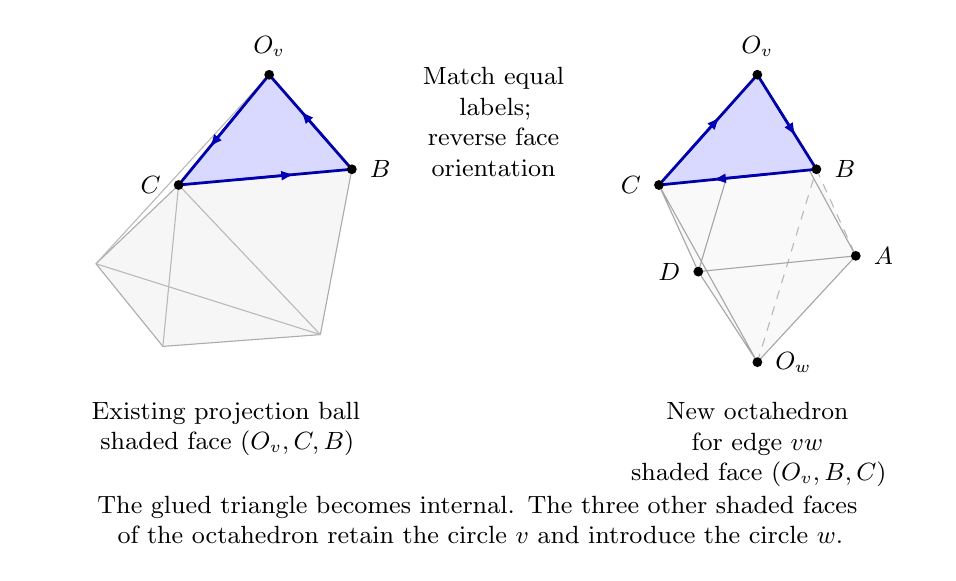
\begin{tikzpicture}[x=1cm,y=1cm,line cap=round,line join=round,
  font=\small,vertex/.style={circle,fill=black,inner sep=1.25pt},
  face/.style={fill=blue!15,draw=blue!65!black,line width=1pt},
  dir/.style={-{Latex[length=1.7mm]},blue!70!black,line width=.85pt}]
\coordinate (ov) at (-3.5,1.85);
\coordinate (b) at (-2.45,.65);
\coordinate (c) at (-4.65,.45);
\coordinate (l) at (-5.7,-.55);
\coordinate (ll) at (-4.85,-1.6);
\coordinate (r) at (-2.85,-1.45);
\fill[gray!7] (ov)--(b)--(r)--(ll)--(l)--(c)--cycle;
\draw[gray!65] (ov)--(b)--(r)--(ll)--(l)--(c)--cycle;
\draw[gray!55] (l)--(r) (ll)--(c) (c)--(r) (ov)--(l);
\path[face] (ov)--(c)--(b)--cycle;
\draw[dir] ($(ov)!.31!(c)$)--($(ov)!.66!(c)$);
\draw[dir] ($(c)!.34!(b)$)--($(c)!.67!(b)$);
\draw[dir] ($(b)!.30!(ov)$)--($(b)!.62!(ov)$);
\foreach \p/\lab/\where in {ov/O_v/above,b/B/right,c/C/left}{
 \node[vertex] at (\p) {};
 \node[\where=3pt] at (\p) {$\lab$};
}
\node[align=center,text width=4.1cm] at (-4.05,-2.65)
 {Existing projection ball\\shaded face $(O_v,C,B)$};
\coordinate (nv) at (2.7,1.85);
\coordinate (nw) at (2.7,-1.8);
\coordinate (na) at (3.95,-.45);
\coordinate (nb) at (3.45,.65);
\coordinate (nc) at (1.45,.45);
\coordinate (nd) at (1.95,-.65);
\fill[gray!5] (nv)--(nb)--(na)--(nw)--(nd)--(nc)--cycle;
\draw[gray!55,dashed] (nw)--(nb) (nb)--(na);
\draw[gray!70] (nv)--(na)--(nw)--(nd)--(nv)
 (nv)--(nb)--(nc)--(nv) (nc)--(nd) (nd)--(na) (nc)--(nw);
\path[face] (nv)--(nb)--(nc)--cycle;
\draw[dir] ($(nv)!.31!(nb)$)--($(nv)!.65!(nb)$);
\draw[dir] ($(nb)!.32!(nc)$)--($(nb)!.66!(nc)$);
\draw[dir] ($(nc)!.29!(nv)$)--($(nc)!.62!(nv)$);
\foreach \p/\lab/\where in {nv/O_v/above,nw/O_w/right,na/A/right,nb/B/right,nc/C/left,nd/D/left}{
 \node[vertex] at (\p) {};
 \node[\where=3pt] at (\p) {$\lab$};
}
\node[align=center,text width=4.1cm] at (2.7,-2.85)
 {\mbox{New octahedron}\\for edge $vw$\\shaded face $(O_v,B,C)$};
\node[fill=white,inner sep=3pt,align=center,text width=2.3cm]
 at (-.65,1.25) {Match equal labels;\\reverse face orientation};
\node[align=center,text width=11.2cm] at (-.85,-3.8)
 {The glued triangle becomes internal. The three other shaded faces of the
 octahedron retain the circle $v$ and introduce the circle $w$.};
\end{tikzpicture}

\caption{One terminal insertion in one projection copy. The old
shaded triangle $(O_v,C,B)$ is identified with $(O_v,B,C)$ in the new
octahedron. The other three shaded faces are those in
\eqref{ctg:oct-faces}; the white sectors follow the two strand-strip
replacements in \eqref{ctg:right-insertion}. The same operation in the
other projection copy gives the two-octahedron block of edge $vw$.}
\label{ctg:attachment-figure}
\end{figure}

\subsection{The primitive collar}
\label{ctg:collar-topology}
On the auxiliary torus the $d_v$ blocks supply $d_v$ annular sectors.
Every page boundary is the same primitive disk longitude $\lambda_v$.
The original meridian crosses these sectors once, in their cyclic
order. A terminal insertion subdivides a passage into two consecutive
passages; it adds neither winding nor a second longitude.
Equivalently, the new triangular interface appears as a transition
and its inverse in the concatenated face word. They cancel, leaving
one primitive transverse passage and the distinguished original disk
map. Locally the two rectangles of a crossing-circle collar identify
opposite sides once. Their side curves are $\mu_v,\lambda_v$, hence
their intersection is one. For an odd seam one endpoint identification
is shifted, but the two rectangles and their once-crossing paths are
retained. Section~\ref{ctg:words} computes those two odd words rather
than replacing the shift by an integral half longitude.

\section{A holomorphic two-octahedron block}
\label{ctg:blocks}

The two-leaf closure is $C(h_0T(h_1))$. Normalize a leaf quadrilateral
to $(0,\infty,1,R)$ and its auxiliary apex to $Z$. In the other
projection copy the apex is $Z/E$, where
\begin{equation}\label{ctg:leaf-coordinates}
 Z=\frac{1+E}{1+H},\qquad
 R=\frac{H(1+E)^2}{E(1+H)^2},\qquad
 Z^2-(1+E)Z+ER=0.
\end{equation}
Here $E,H$ are free complex parameters near $\ii,1$. The two copy
coordinates are holomorphic, not complex conjugates. The normalized
turn and closing maps are
\begin{equation}\label{ctg:turn-close}
 T(z)=\frac{R_1-1}{z-1},\qquad C(z)=\frac{z-R}{z-1},\qquad R_1=1-R.
\end{equation}
They follow by prescribing the images of the three labeled vertices
of the turned and closing faces. Both maps are required to place the
second leaf.

For longitude parameters $t,u$, put
\begin{equation}\label{ctg:angular-coordinates}
\begin{gathered}
 y=\tan(t/2),\quad z=\tan(u/2),\quad
 k=(1+y^2+z^2)^{-1/2},\quad k(0,0)=1,\\
 E=\frac{1+\ii k}{1-\ii k},\quad
 H_0=\frac{1-ky}{1+ky},\quad H_1=\frac{1-kz}{1+kz},\\
 R=\frac{1+z^2}{2+y^2+z^2},\quad R_1=1-R,\qquad
 Z_j=\frac{1+E}{1+H_j}.
\end{gathered}
\end{equation}
Substitution gives \eqref{ctg:leaf-coordinates} for the first leaf,
and its $R_1$ version for the second. Moreover
\begin{equation}\label{ctg:Q}
 Q_j=\frac{E-Z_j}{Z_j-1}=\frac{1+\ii\tan(\tau_j/2)}
                                     {1-\ii\tan(\tau_j/2)}
       =e^{\ii\tau_j},\qquad (\tau_0,\tau_1)=(t,u).
\end{equation}
Thus these formulas prescribe the longitude multipliers exactly.
One can also solve the matching directly: the two normalized base
ratios are
\[
 \kappa_j=\frac{k^2(1+\tan^2(\tau_j/2))}
                         {1-k^2\tan^2(\tau_j/2)}.
\]
Their product is one precisely on the branch
$(k^2+1)((1+y^2+z^2)k^2-1)=0$ through $k=1$.
There $\kappa_0=(1+y^2)/(1+z^2)$ and the two ordered bases are
complementary. This verifies the gluing rather than imposing a
stationary quantum equation.

The octahedra share the equator $q=(0,\infty,1,R)$ and have apices
\begin{equation}\label{ctg:apices}
\begin{array}{c|cc}
 &A&B\\\hline
 +&Z_0& RZ_1/(Z_1-R_1)\\
 -&Z_0/E& RZ_1/(Z_1-ER_1).
\end{array}
\end{equation}
The second column follows by composing the two maps in
\eqref{ctg:turn-close}. At zero the rows are respectively
$((1+\ii)/2,(1-\ii)/2)$ and their reversal.

\begin{lemma}\label{ctg:positive-chart}
For $|t|,|u|\le10^{-2}$ each block is triangulated by eight positive
ideal tetrahedra, whose shapes satisfy $|w-\ii|<0.4$.
Their face maps and internal edge returns are holomorphic throughout
this bidisk.
\end{lemma}

\begin{proof}
We use the standard orientation of upper half-space and the positive
ordered model $(0,\infty,1,w)$, with cross ratio
\begin{equation}\label{ctg:positive-cross-ratio}
 w(a_0,a_1,a_2,a_3)=
 \frac{(a_3-a_0)(a_2-a_1)}{(a_3-a_1)(a_2-a_0)}.
\end{equation}
For the plus copy take ordered tetrahedra
$(B_+,A_+,q_j,q_{j+1})$, $j$ modulo four; for the minus copy take
$(B_-,A_-,q_{j+1},q_j)$. The numerical shape in either case is the
edge cross ratio
\begin{equation}\label{ctg:edge-ratio}
 [a,b,c,d]=\frac{(a-c)(b-d)}{(a-d)(b-c)}
\end{equation}
on the tuple with its first two entries reversed. All eight complete
shapes are $\ii$. This distinction between a tetrahedron's orientation
and the edge-ratio convention will also be used in the seam table.
The diagonal between the two apices divides the original two-pyramid
union into these four tetrahedra in each copy.

Elementary sine and cosine estimates give
$|y|,|z|<0.005001$, hence
\[
\begin{gathered}
 |y^2+z^2|<0.000051,\quad |k-1|<0.000026,\quad
 |E-\ii|<0.00006,\\
 |H_j-1|<0.0102,\qquad |R-\tfrac12|<0.000026.
\end{gathered}
\]
Equation~\eqref{ctg:angular-coordinates} gives
$|Z_j-(1+\ii)/2|<0.004$. Each denominator in the last column of
\eqref{ctg:apices} has complete modulus $1/2$ and changes by less
than $0.0041$. Every finite apex therefore moves by less than $0.02$.
Every complete difference between distinct finite vertices occurring
in a shape has modulus at least $1/2$. Each difference factor changes
by relative size less than $0.08$, so
\[
 |w-\ii|\le
 \frac{4(0.08)+2(0.08)^2}{(1-0.08)^2}<0.4.
\]
Factors involving infinity only shorten this estimate. Thus the
vertices stay distinct and the tetrahedra stay positive. The product
of the four shapes around the apex diagonal telescopes; the total
angle is $2\pi$ on the branch through the regular octahedron.
For complex $t,u$ the equatorial quadrilateral need not lie in one
plane. Its retained triangular boundary and tetrahedral subdivision
are the geometric cells used here.
\end{proof}

\subsection{The full disk-side boundary maps}
The four white transitions of one leaf are
\begin{equation}\label{ctg:white}
\begin{aligned}
 W_0&=\begin{pmatrix}1&0\\0&E\end{pmatrix},&
 W_1&=\begin{pmatrix}1&E-1\\0&E\end{pmatrix},\\
 W_2&=\begin{pmatrix}E-R&R(1-E)\\E-1&1-ER\end{pmatrix},&
 W_3&=\begin{pmatrix}R&0\\1-E&ER\end{pmatrix}.
\end{aligned}
\end{equation}
Matrices act projectively. Each is the unique map of its three labeled
face vertices. For example $W_0(Z)=W_2(Z)=Z/E$ by
\eqref{ctg:leaf-coordinates}. Across a shaded triangle, the white
transition transports the triangle from the other projection copy.
Put $Q=(E-Z)/(Z-1)$. The incoming triangle has cyclic vertices
$(Z,\infty,1)$; the outgoing one has $(Z,R,0)$. Their doubled
two-triangle disk-side boundaries have edge ratios
\begin{equation}\label{ctg:pants}
\begin{array}{c|ccc}
 \text{incoming edge}&(Z,\infty)&(\infty,1)&(1,Z)\\\hline
 \text{ratio}&-Q^{-1}&-Q&-Q^{-1}\\[1mm]
 \text{outgoing edge}&(Z,R)&(R,0)&(0,Z)\\\hline
 \text{ratio}&-Q&-Q^{-1}&-Q.
\end{array}
\end{equation}
Here the ratio of an oriented edge $(a,b)$ with adjacent third
vertices $c,d$ means \eqref{ctg:edge-ratio}. The first entry is
$(1-Z)/(E-Z)=-Q^{-1}$. For the incoming base the opposite apex is
$W_1^{-1}(Z/E)=Z-E+1$; for the outgoing base it is
$W_3^{-1}(Z/E)=ER/(2E-Z)$. These substitutions give the other base
entries; the remaining entries follow from $W_0,W_2$ in the same way.

The complete complex ratios, including their shears, depend only on
$Q=e^{\ii\tau_v}$, not on the parameter at the other end of the edge.
Outgoing and incoming boundaries therefore have inverse ratios under
their original puncture matching. Normalize one triangle by its three
ordered vertices. The ratio table then fixes the other triangle, so
it identifies the whole boundary map. The main puncture products are
one, and the auxiliary puncture product is $Q^{\pm2}$ according to
boundary orientation. The original longitude will have multiplier
$Q^2$.

\subsection{Disk words, signs, and logarithmic increments}
\label{ctg:words}
The pure shaded map and the two cross-copy maps are
\begin{equation}\label{ctg:shaded}
 S=\begin{pmatrix}0&-ER\\1&-1-E\end{pmatrix},\quad
 A=\begin{pmatrix}R&-R\\1&ER-1-E\end{pmatrix},\quad
 B=\begin{pmatrix}R/E-1-1/E&R\\-1&R\end{pmatrix}.
\end{equation}
The pure map sends $(Z,\infty,1)$ to $(Z,0,R)$ within one copy.
The odd maps send respectively
\[
 A:(Z,\infty,1)\mapsto(Z/E,R,0),\qquad
 B:(Z,R,0)\mapsto(Z/E,\infty,1).
\]
The reversal of the two punctures is the literal half-twist disk
identification. Put $\bar S=S|_{E\mapsto E^{-1}}$. Direct
multiplication, using $ER=Z(1+E-Z)$, gives the pure returns
\begin{equation}\label{ctg:pure-returns}
 W_0S=\bar S W_0,\qquad W_2S=\bar S W_2,
 \qquad W_3S=\bar S W_1
\end{equation}
projectively, and the odd returns
\begin{equation}\label{ctg:odd-returns}
 W_0^{-1}BW_2^{-1}A=I,\quad
 W_2^{-1}BW_0^{-1}A=I,\quad
 W_1^{-1}BW_3^{-1}A=I
\end{equation}
projectively. The respective scalar representatives in
\eqref{ctg:odd-returns} are $-R/E,-R/E,(R-1)/E$ times the identity.
These equations check complete edge maps, not just multipliers.
Transport to a common ordered pants chart by \eqref{ctg:pants}
gives the same specified odd seam for incident blocks with different
far-end parameters. No arbitrary permutation of pants punctures is
used.

For clarity, send the auxiliary flag $Z$ to infinity. If a matrix
$M$ fixes $Z$, its affine multiplier there is
$(M_{21}Z+M_{22})^2/\det M$, the reciprocal of its derivative at $Z$.
Set $\rho=Z/(1+E-Z)=H^{-1}$. The two-rectangle paths of
Section~\ref{ctg:collar-topology} are the following words:
\begin{equation}\label{ctg:primitive-words}
\begin{array}{c|c|c}
 \text{curve}&\text{word}&\text{multiplier at infinity}\\\hline
 \lambda&W_2^{-1}W_0&Q^2\\
 \mu\ (\epsilon=0)&S^{-1}&\rho\\
 \mu\ (\epsilon=-1)&A^{-1}W_0&\rho Q\\
 \mu\ (\epsilon=+1)&W_0^{-1}B&\rho/Q.
\end{array}
\end{equation}
All words fix $Z$, and the displayed multiplier formula verifies each
entry algebraically. To read their signs topologically, start on the
incoming disk rectangle, follow the meridian through its first side,
and return across the white side. The negative half twist uses the
inverse $A$ passage followed by $W_0$; the positive half twist uses
$B$ followed by $W_0^{-1}$. The longitude runs across $W_0$ and
returns across $W_2$. The paths cross once, as before insertion.
This is also an explicit convention for the positive crossing $R$ in
\eqref{ctg:powers}. Reversing a physical disk frame transports these
words and its signed crossing together.

The logarithm of the pure local multiplier is
\begin{equation}\label{ctg:increment}
 \log\rho=-\log H_0
 =2\artanh(ky)
 =2\arsinh\!\left(\tan(t/2)\cos(u/2)\right)
 =-2\pi\psi_t(t,u).
\end{equation}
The middle equality uses
$ky=y/\sqrt{1+y^2+z^2}$ and the branches at zero.
Thus \eqref{ctg:psi} has a direct peripheral meaning, independent of
a source action. Concatenating the $d_v$ page increments cancels
changes of intermediate pants frames. The distinguished disk word
adds exactly $-\epsilon_v\log Q_v$, giving the first two equations
of \eqref{ctg:periods}. These are initially chosen logarithms of the
actual multipliers. Section~\ref{ctg:actual-periods} proves that they
are the full log-link periods along the entire path.

\section{A uniform solution of the filling equations}
\label{ctg:contraction}

Write
\begin{equation}\label{ctg:error}
\begin{gathered}
 F(t,u)=2\arsinh\!\left(\tan(t/2)\cos(u/2)\right),\qquad
 E_0(t,u)=F(t,u)-t,\\
 Q_0(t,u)=\sqrt{1-\sin^2(t/2)\sin^2(u/2)}.
\end{gathered}
\end{equation}
The subscript distinguishes these functions from the leaf coordinates
$E,Q$. The square root is one at zero. Differentiation gives
\begin{equation}\label{ctg:derivatives}
 F_t=\frac{\cos(u/2)}{\cos(t/2)Q_0},\qquad
 F_u=-\frac{\sin(t/2)\sin(u/2)}{Q_0}.
\end{equation}
Indeed $1+\tan^2(t/2)\cos^2(u/2)=Q_0^2/\cos^2(t/2)$,
with matching branches at zero. The second derivative in
\eqref{ctg:derivatives} is symmetric in $t,u$, proving the
integrability required by \eqref{ctg:psi}. The action is separately
even and real on real arguments near zero.

\begin{lemma}\label{ctg:error-bound}
On $|t|,|u|\le10^{-2}$, both $|(E_0)_t|$ and $|(E_0)_u|$ are less
than $\delta=1/39000$. Moreover $E_0(t,u)=tH(t,u)$ for a holomorphic
function satisfying $|H|\le\delta$, including at $t=0$.
\end{lemma}

\begin{proof}
Put $a=1/79000$, $b=1/199$, and $\omega=b^4$. With $r=1/200$ the
power-series estimates are
\[
 |\sin(t/2)|\le\frac{r}{1-r^2/6}<b,\qquad
 |\cos(t/2)-1|\le\frac{r^2}{2(1-r^2/12)}<a,
\]
and likewise for $u$. Hence $|Q_0|^{-1}\le(1-\omega)^{-1}$ and
$|Q_0-1|\le\omega$. For the latter use
$(Q_0-1)(Q_0+1)=-\sin^2(t/2)\sin^2(u/2)$ and
$\Rea Q_0>0$. Equation~\eqref{ctg:derivatives} implies the rational
bounds
\begin{equation}\label{ctg:rational-bounds}
 |(E_0)_t|\le\frac{2a/(1-a)+\omega}{1-\omega}<\delta,
 \qquad |(E_0)_u|\le\frac{b^2}{1-\omega}<\delta.
\end{equation}
Since $E_0(0,u)=0$, take
$H(t,u)=\int_0^1(E_0)_t(st,u)\,ds$. This definition is holomorphic
at zero and avoids division by an unknown that might vanish.
\end{proof}

Multiplying \eqref{ctg:charge} by $-2\pi$ gives
\begin{equation}\label{ctg:fixed-equation}
 (d_v-\ii n_v)\tau_v+
       \sum_{w\sim v}E_0(\tau_v,\tau_w)=-2\pi\ii c.
\end{equation}
Define the fixed-point map by solving for the first term. On the
closed polydisk $|\tau_v|\le\rho_0=10^{-2}$ it satisfies, for
complex $|c|\le1$,
\begin{equation}\label{ctg:contraction-bounds}
 |\mathcal T_{c,v}|\le\frac{2\pi}{630}+\delta\rho_0<\rho_0,
 \qquad
 \sum_w|\partial_{\tau_w}\mathcal T_{c,v}|
        \le\frac{2d_v\delta}{L_v}\le2\delta<1.
\end{equation}
The strict radius inequality already follows from $\pi<22/7$.
The contraction theorem gives a unique solution; iteration from zero
converges uniformly in $c$. Each iterate is holomorphic, so the
solution is holomorphic. The strict radius margin allows
$|c|\le1+\eta$ for some $\eta>0$, proving the neighborhood statement
in Theorem~\ref{ctg:main}.

Its sign is an additional fact, not a consequence of smallness.
Equation~\eqref{ctg:fixed-equation} is
\begin{equation}\label{ctg:denominator}
 A_v\tau_v=-2\pi\ii c,\qquad
 A_v=d_v-\ii n_v+\sum_{w\sim v}H(\tau_v,\tau_w).
\end{equation}
For real $c>0$,
\begin{equation}\label{ctg:sign}
 \Rea A_v\ge(1-\delta)d_v>0,\qquad
 \Ima\tau_v=-\frac{2\pi c\,\Rea A_v}{|A_v|^2}<0,
 \qquad |A_v|\ge L_v-\delta d_v.
\end{equation}
This proves \eqref{ctg:tau-bound}. It divides by neither $n_v$ nor
$\tau_v$, and works with mixed signs and zero powers. Substituting
\eqref{ctg:powers} and \eqref{ctg:charge} in the peripheral formulas
now gives $U_v+p_vV_v=-2\pi\ii c$ as an equality of chosen logs.

\section{The metric and the full primitive periods}
\label{ctg:metric}

Realize each edge block by Lemma~\ref{ctg:positive-chart}, and glue its
pages in the order of Proposition~\ref{ctg:cut}. Table~\eqref{ctg:pants}
matches full complex shears, not just dihedral angles. Equations
\eqref{ctg:pure-returns} and \eqref{ctg:odd-returns} check the disk
edge returns. At every edge the angle branch is $2\pi$, by positivity
and continuation from the regular cells. Thus finite points have
nonsingular hyperbolic neighborhoods. If an auxiliary subdivision
uses a finite vertex, its topological sphere link has a nonsingular
spherical metric; its complete spherical development is the ordinary
sphere. No global injectivity of the developing map is needed here.

The horospherical triangles give a nonsingular similarity structure on
each topological cusp torus. At a main corner the small meridian is
$W_{j-1}^{-1}W_j$, or its inverse in the transported frame. Its
multiplier is one. It remains nontrivial: for example
$W_0^{-1}W_1$ is translation by $E-1$, and the other corner words
are its marked counterparts. The small chart excludes $E=1$.
The commuting peripheral maps therefore are translations at this
parabolic flag. The compact link is a Euclidean torus, so the main
cusps are complete.

At an auxiliary end and real $c>0$,
\begin{equation}\label{ctg:nonunit}
 \Rea V_v=-2\Ima\tau_v>0.
\end{equation}
The peripheral group has a nonunit dilation and hence a second common
fixed point $q_v$ in the affine chart whose first flag is infinity.
Its similarity development misses $q_v$. Indeed the invariant vector
field $(z-q_v)\partial_z$ descends to the torus. Any zero has index
$+1$, because the developing map is locally orientation-preserving.
The Euler characteristic of the torus is zero, so there are no zeros.

On the simply connected link cover define
\begin{equation}\label{ctg:log-link}
 f_v=\log(\operatorname{dev}_v-q_v).
\end{equation}
Its real derivative is invertible. The metric $|df_v|^2$ descends to a
nonsingular Euclidean metric on the compact torus and is complete.
Lifting geodesics makes $f_v$ a covering of the Euclidean plane, and
therefore a diffeomorphism. Its two generator periods form an injective
real rank-two lattice.

\subsection{Fixing the winding integer}
\label{ctg:actual-periods}
Let $P_{\mu_v},P_{\lambda_v}$ be the periods of \eqref{ctg:log-link}
along the original primitive paths. Their exponentials are the
multipliers already computed, so
\begin{equation}\label{ctg:integer-periods}
 P_{\mu_v}-U_v,\ P_{\lambda_v}-V_v\in2\pi\ii\mathbb Z.
\end{equation}
The integers are continuous for $0<c\le1$: the link is nonsingular,
the paths and flags are retained, and a base logarithm can be continued.
Rebasing changes no period.

To determine the integers, use a continuous frame sending the chosen
flag to infinity. The longitude is $z\mapsto a(c)z+b(c)$ with
$a=e^{V_v}$, $a(0)=1$, and $b(0)\ne0$. The last inequality follows
from the original primitive longitude in the complete Euclidean torus.
Its second fixed point is $q_v=b/(1-a)$; hence $|q_v|\to\infty$ as
$c\downarrow0$. The fixed-generator paths use finitely many triangles
and continuous transition maps, so their images are bounded by some
$B$ and their Euclidean lengths by some $L$ for this fixed tree. Thus
\begin{equation}\label{ctg:period-limit}
 |P_\gamma(c)|\le\frac{L}{|q_v(c)|-B}\longrightarrow0.
\end{equation}
Also $U_v,V_v\to0$. The integers in \eqref{ctg:integer-periods}
vanish near zero and hence along the whole path. In particular the
actual primitive filling slope has period $-2\pi\ii c$ even if the
sum of its many small page contributions is close to $-2\pi\ii$.
No principal logarithm is reset.

\subsection{Adding the core}
Send the fixed points to zero and infinity. In upper half-space write
$r=y/|z|$, and use coordinates
\begin{equation}\label{ctg:tube-coordinates}
 R_*=\arsinh(1/r),\qquad \theta=\Ima f_v,\qquad
 X=\Rea f_v+\tfrac12\log(1+r^2).
\end{equation}
A direct substitution into $y^{-2}(|dz|^2+dy^2)$ gives
\begin{equation}\label{ctg:tube-metric}
 dR_*^2+\cosh^2R_*\,dX^2+\sinh^2R_*\,d\theta^2.
\end{equation}
The original ideal end contains all sufficiently high vertical rays
over its finitely many similarity triangles. Compactness of their
quotient gives a whole punctured tube $0<R_*<R_0$ in these coordinates.
The primitive slope $\mu_v+p_v\lambda_v$ has zero real period and
angular period $-2\pi c$. Its complementary curve is $\lambda_v$,
because the change of primitive basis has determinant one. That curve
has positive real period $\ell_v=\Rea V_v$.

Adding $R_*=0$ gives a cone solid torus of angle $2\pi c$ and core
length $\ell_v$. At $c=1$ it is a smooth solid torus with precisely
the original filling meridian. Main cusps are still complete horoball
quotients and the middle is compact. Hence the resulting smooth metric
is complete and has finite volume on $Y(\mathbf p)$. Its universal
local development covers simply connected hyperbolic space and is an
isometry; this is the geometric holonomy of the original filled
exterior. For $c<1$ we assert a cone metric, not a smooth filled-group
representation or discreteness of its holonomy.

\begin{figure}[t]
\centering
% Logarithmic peripheral periods, with p=2 in the drawn lattice.
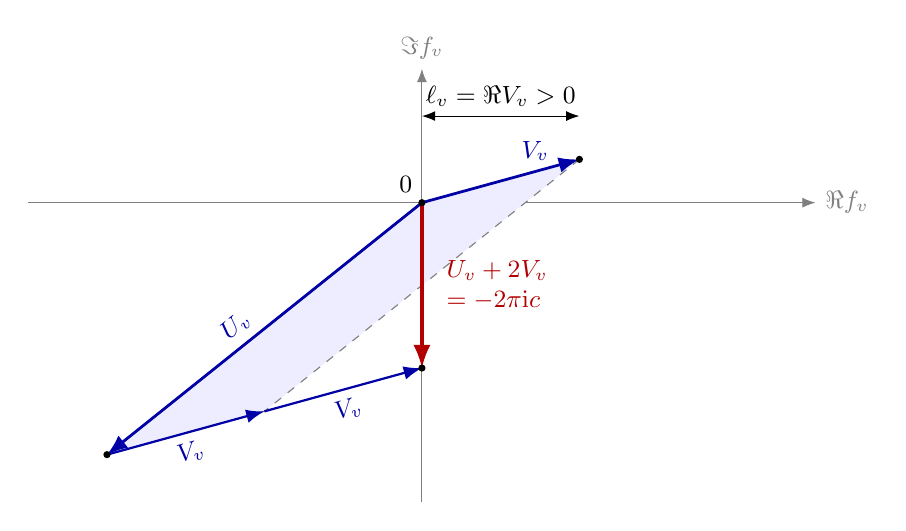
\begin{tikzpicture}[x=1cm,y=1cm,>=Latex,font=\small]
 \draw[->,gray] (-5,0)--(5,0) node[right] {$\Re f_v$};
 \draw[->,gray] (0,-3.8)--(0,1.7) node[above] {$\Im f_v$};
 \coordinate (O) at (0,0);
 \coordinate (V) at (2,.55);
 \coordinate (U) at (-4,-3.2);
 \coordinate (S) at (0,-2.1);
 \fill[blue!7] (O)--(V)--(-2,-2.65)--(U)--cycle;
 \draw[gray,dashed] (V)--(-2,-2.65)--(U);
 \draw[->,line width=1pt,blue!65!black] (O)--(V)
    node[pos=.72,above] {$V_v$};
 \draw[->,line width=1pt,blue!65!black] (O)--(U)
    node[pos=.55,above,sloped] {$U_v$};
 \draw[->,line width=.8pt,blue!65!black] (U)--(-2,-2.65)
    node[midway,below,sloped] {$V_v$};
 \draw[->,line width=.8pt,blue!65!black] (-2,-2.65)--(S)
    node[midway,below,sloped] {$V_v$};
 \draw[->,line width=1.2pt,red!70!black] (O)--(S)
    node[midway,right=5pt,align=left] {$U_v+2V_v$\\$=-2\pi\ii c$};
 \draw[<->] (0,1.1)--(2,1.1)
    node[midway,above] {$\ell_v=\Re V_v>0$};
 \foreach \p in {O,V,U,S}{\fill (\p) circle (1.3pt);}
 \node[above left] at (O) {$0$};
\end{tikzpicture}

\caption{The auxiliary log-link plane for $c>0$. The lattice generators
are the full periods $V_v$ and $U_v$. Their primitive combination
$U_v+p_vV_v=-2\pi\ii c$ is the angular meridian; $V_v$ supplies the
positive core translation. The diagram shows $p_v=2$ for the period
relation only. The real period of the slope vanishes, and its angular
period reaches exactly one turn at $c=1$.}
\label{ctg:period-figure}
\end{figure}

\section{Absolute volume and core estimates}
\label{ctg:regulator}

We state precisely the local companion fact used in this section.
For an oriented positive ideal triangulation of a torus-ended
3-manifold, suppose the full face and edge gluing equations hold and
$U_i,V_i$ are continued affine similarity logarithms along primitive
oriented torus bases. The sum $\mathcal V_\rho$ of the oriented
tetrahedral volumes satisfies
\begin{equation}\label{ctg:volume-differential}
 d\mathcal V_\rho=\frac12\sum_i
   \bigl(\Rea V_i\,d\Ima U_i-\Rea U_i\,d\Ima V_i\bigr).
\end{equation}
This is the local identity proved in \cite[Section~7]{MarkedFillings},
equation (7.3); it does not assume that the
ends are complete or that the total logs are small. Its convention is
the positively ordered model and cross ratio
\eqref{ctg:positive-cross-ratio}. For one tetrahedron its proof starts
from the Bloch--Wigner differential
\[
 dD(w)=\log|w|\,d\arg(1-w)-\log|1-w|\,d\arg w.
\]
On the cusp triangles, the side-scale transitions telescope along the
actual normal paths. The peripheral coefficient rows pair to minus
twice their oriented intersection; after quotienting the isotropic
edge rows the tangent pairing is $-\tfrac12\sum_i dU_i\wedge dV_i$.
These two identities give \eqref{ctg:volume-differential} for similarity
logs. They are local chain identities and continue along a positive
family. The classical framework appears in Neumann--Zagier
\cite{NeumannZagier}.

The orientation of the primitive basis can also be checked directly
in its exact complete coordinates. In the affine chart
$h(z)=1/(z-Z)$, with $E=\ii$, $R=1/2$, and $Z=(1+\ii)/2$, the
words $S^{-1}$ and $W_2^{-1}W_0$ translate by $1-\ii$ and
$2+2\ii$. The negative and positive odd meridians translate by
$2$ and $-2\ii$. Consequently the $d_v$-page collar has translations
\[
 \mu_v:\ d_v(1-\ii)-\epsilon_v(1+\ii),\qquad
 \lambda_v:\ 2(1+\ii),\qquad
 \Ima\frac{\lambda_v}{\mu_v}
             =\frac{2d_v}{d_v^2+\epsilon_v^2}>0.
\]
This fixes the same oriented primitive-basis convention used in
\eqref{ctg:volume-differential}. Here the quotient denotes the ratio
of the displayed translation vectors, not a quotient of curves.

Here all hypotheses have been verified: Proposition~\ref{ctg:cut}
identifies the oriented manifold and primitive paths;
Lemma~\ref{ctg:positive-chart} gives positive oriented tetrahedra;
\eqref{ctg:pants}--\eqref{ctg:odd-returns} supply complete edge
returns; and Section~\ref{ctg:actual-periods} fixes the logarithmic
lifts. Main meridians have $U=0$ and contribute zero. Thus the
companion's local differential applies to this whole path, without
using its separate long-filling existence theorem.

Put $U_v^0=-2\pi\Psi_{\tau_v}$ and define
\begin{equation}\label{ctg:G}
\begin{split}
 G^0&=2\pi\ii\left(\Psi-\sum_v\tau_v\Psi_{\tau_v}\right),\qquad
 dG^0=\tfrac12\sum_vV_v\,dU_v^0,\\
 G&=G^0-\sum_v\frac{\epsilon_vV_v^2}{8}
   =2\pi\ii\left(\Psi-\sum_v\tau_v\Psi_{\tau_v}\right)
                          +\sum_v\frac{\epsilon_v\tau_v^2}{2}.
\end{split}
\end{equation}
Thus $dG=\tfrac12\sum_vV_vdU_v$. Differentiating and using
\eqref{ctg:volume-differential} shows that
\begin{equation}\label{ctg:absolute-regulator}
 \mathcal V_\rho=\Ima G-\tfrac12\sum_v\Rea U_v\,\Ima V_v.
\end{equation}
The constant is fixed at the complete assembly: its $2e$ regular
octahedra have volume $2e v_{\rm oct}=2\pi\Psi(0)=\Ima G(0)$.
Every shape remains in a simply connected positive neighborhood of
$\ii$, so no volume or logarithmic branch is reset.

\subsection{The same fundamental chain computes metric volume}
Equality \eqref{ctg:absolute-regulator} is not by itself an
identification with filled metric volume. We make that comparison on
the same eight-tetrahedron chain at each original tree edge.
At an auxiliary end send its fixed points to zero and infinity, and
retain one finite boundary triangulation. Let $w$ range over a fixed
fundamental cross section and let $Y\to\infty$ be a height parameter.
The ideal conical map has the form $(a(w),Yb(w))$, where $b>0$.
The logarithmic link supplies a real function $\eta$ whose deck
increments are the real peripheral periods. The axis-valued map
$(0,Ye^{\eta(w)})$ is equivariant. Compare them by
\begin{equation}\label{ctg:homotopy}
 H_s(w,Y)=\left(sa(w),Y\exp\bigl((1-s)\eta(w)+s\log b(w)\bigr)\right),
 \qquad 0\le s\le1.
\end{equation}
The assignments agree on shared boundary faces. They are equivariant
because $a$, $b$, and $e^\eta$ transform by the complex multiplier,
its modulus, and its modulus, respectively. On the compact cross
section the horizontal derivatives are bounded, the height is
comparable to $Y$, and its derivatives are $O(Y)$. The hyperbolic
volume form $y^{-3}dx_1\wedge dx_2\wedge dy$ therefore bounds the
boundary homotopy volume by $O(Y^{-2})$.

For fixed $0<c\le1$ this compares the ideal chain with the metric
away from the cone axis; the axis has zero three-dimensional volume.
At $c=1$ the actual primitive meridian has period $-2\pi\ii$ and
zero real period, so the axis assignment extends over its meridian
disk. Extend the same boundary triangulation through the solid torus
with added vertices on the axis. All added tetrahedra have zero
volume. The main horoball comparisons likewise have vanishing
boundary volume. Stokes' theorem on the common truncated chain and
the limit in \eqref{ctg:homotopy} give
\begin{equation}\label{ctg:chain-volume}
 \mathcal V_\rho=\Vol_c.
\end{equation}
For $c<1$ this is a comparison on the cone metric away from its axis,
not an assertion of smooth group descent. At $c=0$ it follows by
continuity of the positive tetrahedral volumes.

At the critical point let $\Phi=G/(2\pi\ii)$. The equations
\eqref{ctg:charge} and $n_v=\epsilon_v-2p_v$ give
\begin{equation}\label{ctg:cancellation}
 \Phi-\calC(c)=-\frac{\ii}{2\pi}\sum_vp_v\tau_v^2,
 \qquad
 \tfrac12\Rea U_v\,\Ima V_v=p_v\Ima(\tau_v^2).
\end{equation}
Substituting into \eqref{ctg:absolute-regulator} and
\eqref{ctg:chain-volume} cancels the boundary correction and proves
\eqref{ctg:volume}. This completes Theorem~\ref{ctg:main}.

\begin{corollary}\label{ctg:quantitative-volume}
Let $S_{\mathcal T}=\sum_v d_v/L_v^2$. Under Theorem~\ref{ctg:main},
\begin{equation}\label{ctg:core-bounds}
 \frac{4\pi c(1-\delta)d_v}{(L_v+\delta d_v)^2}
 \le\ell_v(c)\le
 \frac{4\pi c(1+\delta)d_v}{(L_v-\delta d_v)^2},
\end{equation}
and
\begin{equation}\label{ctg:loss-bounds}
 \frac{2\pi^2(1-\delta)}{(1+\delta)^2}S_{\mathcal T}
 \le 2e v_{\rm oct}-\Vol(Y(\mathbf p))\le
 \frac{2\pi^2(1+\delta)}{(1-\delta)^2}S_{\mathcal T}.
\end{equation}
\end{corollary}
\begin{proof}
In \eqref{ctg:denominator},
$(1-\delta)d_v\le\Rea A_v\le(1+\delta)d_v$ and
$L_v-\delta d_v\le|A_v|\le L_v+\delta d_v$.
Equation~\eqref{ctg:sign} gives \eqref{ctg:core-bounds}.
Stationarity in \eqref{ctg:action} gives
\[
 \frac{d}{dc}\Vol_c=2\pi\sum_v\Ima\tau_v(c)
                         =-\pi\sum_v\ell_v(c).
\]
Integrate from $0$ to $1$, and use $d_v\le L_v$ in the
denominators. This proves \eqref{ctg:loss-bounds}.
The derivative also agrees with the Schläfli expression
$-\tfrac12\sum_v\ell_v\,d(2\pi c)$; it is a normalization check,
not the argument fixing the absolute constant.
\end{proof}

\section{A criterion with different vertex radii}
\label{ctg:variable-radii}

The common threshold is convenient but is not required by the proof.
The next finite criterion uses the actual neighboring radii.

\begin{theorem}\label{ctg:heterogeneous}
Choose $0<r_v\le10^{-2}$ and define
\begin{equation}\label{ctg:radius-data}
 s_v=\sinh(r_v/2),\quad a_v=\cosh(r_v/2)-1,\quad
 \omega_{vw}=s_v^2s_w^2,
\end{equation}
\begin{equation}\label{ctg:alpha-beta}
 \alpha_{vw}=\frac{a_v+a_w}{(1-a_v)\sqrt{1-\omega_{vw}}}
                +\frac1{\sqrt{1-\omega_{vw}}}-1,
 \qquad
 \beta_{vw}=\frac{s_vs_w}{\sqrt{1-\omega_{vw}}},
 \qquad h_v=\sum_{w\sim v}\alpha_{vw}.
\end{equation}
Suppose
\begin{equation}\label{ctg:radius-criterion}
 \begin{gathered}
 2\pi+h_vr_v<L_vr_v,\qquad h_v<d_v,\\
 \max_v\left(\frac{h_v}{L_v}
       +\sum_{w\sim v}\frac{\beta_{vw}r_w}{L_vr_v}\right)<1.
 \end{gathered}
\end{equation}
Then the existence, cone completion, smooth endpoint, and absolute
volume conclusions of Theorem~\ref{ctg:main} hold, with uniqueness
in $|\tau_v|\le r_v$ and the bound
\begin{equation}\label{ctg:radius-bound}
 |\tau_v(c)|\le\frac{2\pi c}{L_v-h_v},\qquad \Ima\tau_v(c)<0.
\end{equation}
The last line of \eqref{ctg:radius-criterion} may instead be replaced
by a positive vector $q$ and $\kappa<1$ satisfying $Mq\le\kappa q$,
where $M_{vv}=h_v/L_v$ and $M_{vw}=\beta_{vw}/L_v$ for adjacent
distinct vertices. The invariant-polydisk inequalities in the first
line remain required separately.
\end{theorem}

\begin{proof}
On the corresponding bidisk, \eqref{ctg:derivatives} bounds
$|(E_0)_t|$ by $\alpha_{vw}$ and $|(E_0)_u|$ by $\beta_{vw}$:
use $|\sin(t/2)|\le s_v$, $|\cos(t/2)-1|\le a_v$, and
$|Q_0|\ge\sqrt{1-\omega_{vw}}$. The binomial series also gives
$|Q_0^{-1}-1|\le(1-\omega_{vw})^{-1/2}-1$, which accounts for
the final two terms in $\alpha_{vw}$. Integrating $(E_0)_t$ from zero
gives $|E_0(t,u)|\le\alpha_{vw}|t|$.
The first inequality makes the fixed-point map preserve the product
of the chosen disks. The last is its derivative bound in the norm
$\max_v|\tau_v|/r_v$; alternatively $Mq\le\kappa q$ gives the
$q$-weighted norm. Thus the same uniform iteration proves existence,
uniqueness, and holomorphic dependence near $|c|\le1$.
The denominator now has real part at least $d_v-h_v>0$ and modulus
at least $L_v-h_v$. This proves \eqref{ctg:radius-bound}.
All geometric steps require only these sign and radius bounds, so
Sections~\ref{ctg:metric}--\ref{ctg:regulator} apply unchanged.
\end{proof}

The inequalities are an explicit certificate in the integer degrees,
powers, and chosen positive radii. Rational Taylor enclosures can
verify them; they assume neither a saddle nor a representation.
The contraction calculation itself works for a finite graph, but
the geometric conclusion here uses the ordered tree cut proved in
Proposition~\ref{ctg:cut}. It supplies no geometric identification
for an arbitrary graph with cycles.

\section{Use in filling asymptotics and finite verification}
\label{ctg:scope}

This paper exports a geometric implication: any analysis selecting
the solution of \eqref{ctg:charge} in the stated positive polydisk
may identify its real critical action by \eqref{ctg:volume}.
It does not provide the analysis that selects that branch from an
oscillatory invariant. In particular a tree's Newton polynomial
kernel and its turning factors require their own exact adapter;
they do not follow merely from the abstract finite filling norm.

For reference, the common sufficient conditions in the retained
circle-tree estimates all enter this geometric theorem. If
\[
 \sum_v\frac{d_v}{d_v^2+n_v^2}\le2^{-25},
 \quad\text{or}\quad
 \max_v\frac{d_v}{d_v^2+n_v^2}\le2^{-120},
\]
then respectively $L_v\ge2^{25/2}>630$ or $L_v\ge2^{60}>630$,
since $d_v\ge1$. The directed estimate uses
$D_v=(d_v-\ii n_v)/(2\pi)$ and requires
$2^{-14}|D_v|\ge2$, so $L_v\ge2\pi\,2^{15}>630$.
These observations identify their geometric input; none replaces
the different remainder and noncancellation arguments of those
estimates.

Two existing exact programs check bounded algebra used above:
\nolinkurl{audit_two_octahedron_angular_edge_block.py} checks the
rational pants ratios, odd returns, angular formulas, and positive
chart bounds, while
\nolinkurl{audit_all_circle_vertexwise_geometry.py} checks the
rational inequalities in Lemma~\ref{ctg:error-bound} and
\eqref{ctg:contraction-bounds}. They are in the repository's
\texttt{experiments} directory and accept an explicit output path.
The paper-local driver records their source hashes and results.
These calculations check finite identities and constants; they do
not prove the topological identification, the contraction theorem,
the link covering argument, or the volume comparison. Those are
the written arguments above.

\begin{thebibliography}{9}
\bibitem{MarkedFillings}
\emph{Circle patterns and primitive fillings of augmented links}, companion paper,
Section~7, peripheral-volume differential.
\url{https://sashakolpakov.github.io/murakamis_dream/papers/marked-fillings.pdf}.

\bibitem{Purcell}
J.~S. Purcell, \emph{An introduction to fully augmented links},
Contemporary Mathematics \textbf{541} (2011), 205--220.
\href{https://users.monash.edu/~jpurcell/papers/expos-auglinks.pdf}
{Author's full text}.

\bibitem{BeltedSums}
P.~Morgan, B.~Ransom, D.~Spyropoulos, R.~Trapp and C.~Ziegler,
\emph{Belted sum decompositions of fully augmented links},
New York J. Math. \textbf{31} (2025), 1--42.
\url{https://nyjm.albany.edu/j/2025/31-1.pdf}.

\bibitem{NeumannZagier}
W.~D. Neumann and D.~Zagier,
\emph{Volumes of hyperbolic three-manifolds},
Topology \textbf{24} (1985), 307--332.
\href{https://doi.org/10.1016/0040-9383(85)90004-7}
{doi:10.1016/0040-9383(85)90004-7}.
\end{thebibliography}
\end{document}
